\subsection{The \boldmath$Wtb$ vertex structure in \boldmath$t$-channel single-top-quark production and decay} \label{subsec:Wtb}

%Introp tp top quark%
The top quark is the heaviest elementary particle discovered so far, with a mass of $m_{top}=172.44 \pm 0.13$(stat)$\pm 0.47$(syst)~GeV~\cite{Khachatryan:2015hba}, followed by the Higgs boson, with $m_{H}=125.09\pm0.21$(stat.)$\pm0.11$(syst.)~GeV~\cite{Aad:2015zhl}. In the context of the SM, the top quark is the isospin\footnote{Particles that are identically affected by strong interactions but have different charges can be treated as being different states of the same particle with isospin values related to the number of charge states.} partner of the $b$-quark, which is $35$ times lighter~\cite{Olive:2016xmw}. Due to its large mass, measurements of phenomena involving the top-quark physics are crucial to our understanding of the electroweak sector in the SM or beyond the SM (BSM) theories. 
%Explicación sispín: The isospinis a quantum number related to the strong interaction. Particles that are affected equally by the strong force but have different charges (e.g. protons and neutrons, top-quark and b-quark) can be treated as being different states of the same particle with isospin values related to the number of charge states.
%Trivia: The top-quark is approximately as heavy as an entire atom of gold)

In 1973 M. Kobayashi and T. Maskawa postulated the top quark in order to explain the CP violations in kaon decay~\cite{Kobayashi:1973fv}. It was later discovered in 1995 by the CDF~\cite{PhysRevLett.74.2626} and DØ~\cite{Abachi:1995iq} experiments at Fermilab. The Nobel Prize in Physics 2008~\cite{NobelPrize} was divided in two halves, one half was conceded to Y. Nambu ``for the discovery of the mechanism of spontaneous broken symmetry in subatomic physics" and the other half was shared among M. Kobayashi and T. Maskawa ``for the discovery of the origin of the broken symmetry which predicts the existence of at least three families of quarks in nature".

%Decay of Top Quark%
The top quark decays to a $W$ boson and a down-type quark via flavour changing electroweak processes. The branching ratios (BR) of its decays are related to the Cabibbo-Kobayashi-Maskawa (CKM) matrix elements:
\begin{equation} \label{eq:BRtdecay}
\frac{BR(t \rightarrow Wb)}{BR(t \rightarrow Wq)}= \frac{|V_{tb}|^2}{\sum |V_{tq}|^2} =  |V_{tb}|^2 \approx 1
\end{equation}
where $q$ stands for the three possible quarks to which top quark can decay: $d$, $s$ and $b$. Expression \ref{eq:BRtdecay} means that the top quark decay happens almost always to a $b$-quark and a $W$ boson.

As a consequence of the huge mass of the top quark, its life time is extremely short, $\mathcal{O}(10^{-25}$~s). It is shorter than the time scale of quantum chromodynamics (QCD), $\mathcal{O}(10^{-24}$~s), allowing this quark to be studied as a free quark. Therefore, the top quark decays before hadronising. Moreover, since its lifetime is also shorter than the depolarisation timescale, $\mathcal{O}(10^{-21}$~s)~\cite{Bigi:1986jk}, and the $W$ boson is produced on-shell in the top-quark decay, the top-quark spin information is directly transferred to its decay products. Thus, we can measure its polarisation from its decay products.

% Therefore, the top quark decays before hadronizing. Moreover, we can study the top quark as a free quark and measure its polarisation from its decay products since the spin information is not diluted through the hadronization; the depolariastion scale is of the timescale $\mathcal{O}(10^{-21}$~s)~\cite{Bigi:1986jk}. 
%The top quark's lifetime, $\mathcal{O}(10^{-24}$~s), is extremely short due to its huge mass, and is smaller than the hadronization	scale, $\mathcal{O}(10^{-24}$~s); as such, it is impossible for the top quark to hadronize (i.e. to form bound states). An important consequence is that we can study the top quark as if it were a free quark. Therefore, it is possible to measure its polarisation since the spin information is not diluted through the hadronization; the depolariastion scale is of the timescale $\mathcal{O}(10^{-21}$~s)~\cite{Bigi:1986jk}. 
% When using the "second conditional", it is also correct to use "were" for the first and third person singulars.

The top quark decay is classified in different channels depending on the decay of the $W$ boson. The $W$ boson can decay either leptonically into a lepton and its corresponding antineutrino or hadronically into two quarks ($u\bar{d}$ or $c\bar{s}$). The relative branching ratio:
\begin{equation}
\frac{BR(W\rightarrow q\bar{q})}{BR(W\rightarrow l \bar{\nu})}=\frac{BR(W \rightarrow c\bar{s},u\bar{d})\times colour}{BR(W \rightarrow e,\mu,\tau)}=6/3
\end{equation}
%\begin{equation}
%\frac{hadronically}{leptonically}=\frac{(c\bar{s},u\bar{d})\times colour}{(e,\mu,\tau)}=6/3
%\end{equation}
%(cs,ud) = 2, Colour = 3. 
In the $t$- and $s$-channels, where only one $W$ boson is produced, it is possible to classify two samples: the hadronic and the leptonic one. The leptonic sample includes the leptonic decays of the $W$ boson into electrons, muons or leptonic taus decays, plus their corresponding antineutrinos. On the other hand, the hadronic sample comprises the hadronic $W$-boson decays and the hadronic-tau decays\footnote{The lepton $\tau$ is the only lepton that can decay into hadrons, occurring 64.79\% times. The predominant hadronic decay is into a charged pion, a neutral pion, and a tau neutrino. The non-hadronic decays are into an electron or a muon, occurring 17.82\% and 17.39\% of times respectively~\cite{Olive:2016xmw}, plus their corresponding neutrinos.}.
%TAU DECAY
%Tienes los modos 1-prong ( un pión cargado + neutrinos (+ piones neutros ==> fotones )
%y 3-prong ( tres piones cargados..)
%El modo predominante es 1-prong, y da lugar a un jet muy colimado !
%https://en.wikipedia.org/wiki/Tau_(particle)#Tau_decay
The scope of the presented analysis is the study of the $t$-channel single-top-quark events with the top quark decaying into leptonic $W$ bosons, with an electron in the final state.

% Top quark production%
In hadron colliders there are two production mechanisms of top quark: top-quark pairs ($t\bar{t}$) and single-top quarks. Single-top quarks are produced, at leading order (LO) in QCD perturbation theory, by three different electroweak subprocesses: the exchange of a virtual $W$ boson in the \mbox{$t$-channel} or the \mbox{$s$-channel}, or the case with an on-shell $W$ boson~\cite{Probing} (Figure \ref{Fig:FeynmanSingTopProd}). %the nex-to-next-to-leading order cross sections at $8$ TeV for those mechanisms are (assuming $m_{top}=172.5$ GeV): $\sigma_{t-channel}=87.8_{-1.9}^{+3.4}$ pb, $\sigma_{Wt-channel}=22.4 \pm 1.5$ pb and $\sigma_{s-channel}=5.6 \pm 0.2$ pb~\cite{Kidonakis:2011wy}. 
As can be seen in Table~\ref{Tab:xSections}, the $t$-channel dominates the single-top production.%That is why it is the mechanism in which this dissertation is focused.
 For the $\sqrt{s}=13$~TeV data, the total cross-sections for both top quark and top antiquark production are measured to be $\sigma(tq)=156 \pm 5$(stat.) $\pm 27$(syst.) $\pm 3$(lumi.)~pb and $\sigma(\bar{t}q)=32.9\pm 4$(stat.) $\pm 18$(syst.) $\pm 2$(lumi.)~pb, respectively~\cite{Hirschbuehl:2017veq}~\cite{Aaboud:2016ymp}. The cross-section ratio of top-quark to top-antiquark production is, therefore, $R_t = \frac{\sigma(tq)}{\sigma(\bar{t}q)}= 1.72 \pm 0.09$(stat.) $\pm 0.18$(syst.).
 
\begin{figure}[h]
\centering
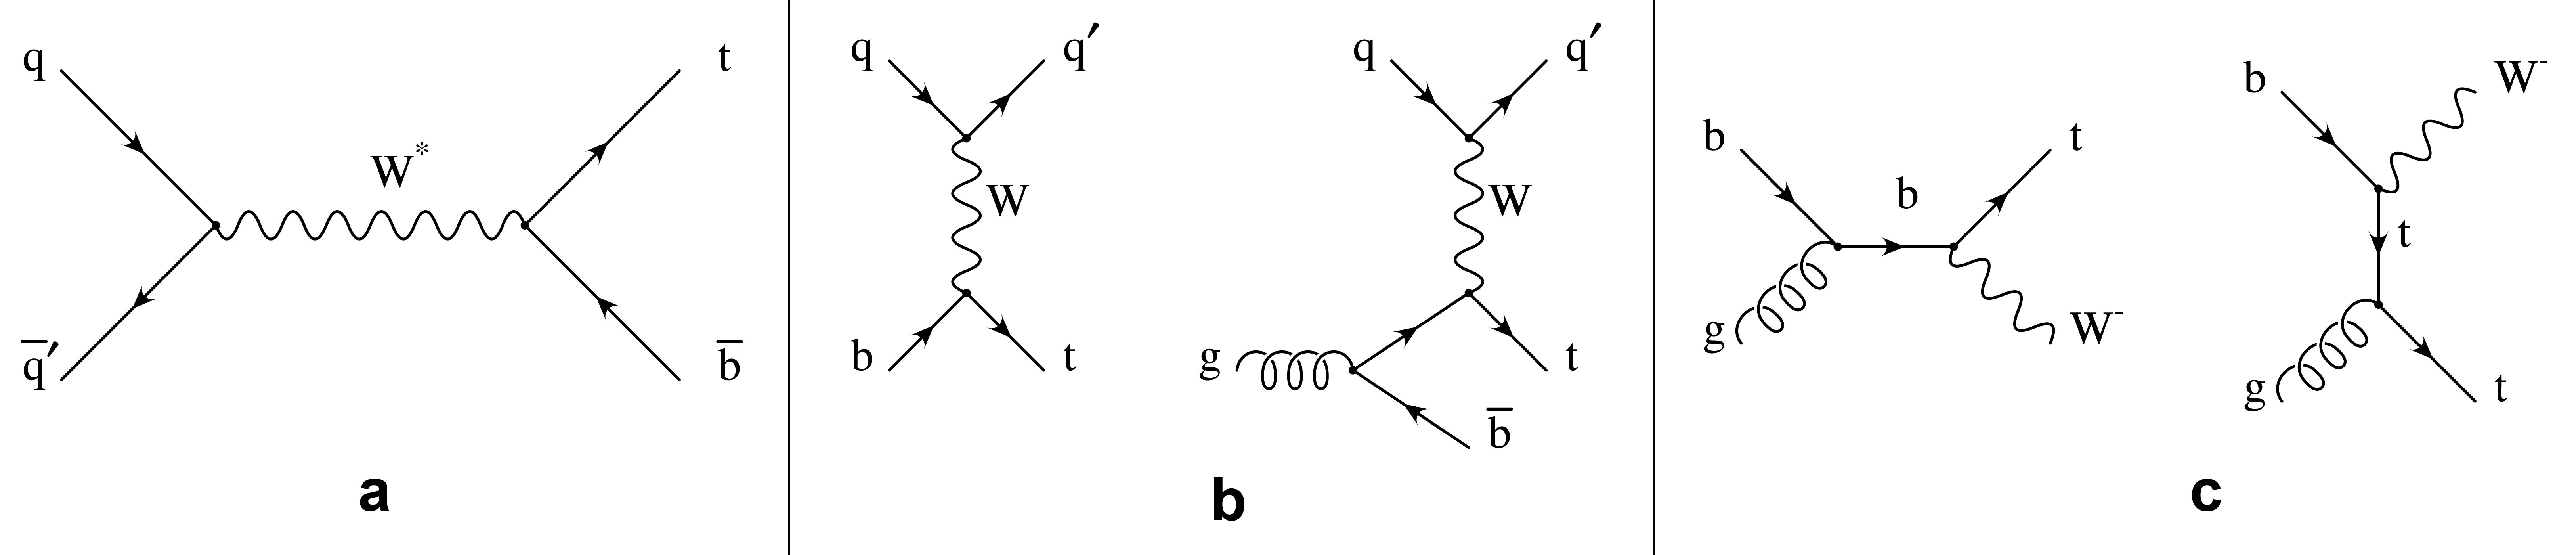
\includegraphics[width=0.95\textwidth]{/afs/ific.uv.es/user/p/pamarag/public/RedaccionTFM/Figuras/single_Top_channels_0.jpg}
\caption{Feynman diagrams for single top quarks production in $pp$ collisions: a) $s$-channel b) $t$-channel c) $Wt$ associated decay.}
\label{Fig:FeynmanSingTopProd}
\end{figure}


\begin{table}
\centering
\begin{tabular}{|c | c c c|} 
 \hline
 $\sqrt{s}$~(TeV)& $\sigma_{t-chan}$ (pb)& $\sigma_{Wt-chan}$ (pb) & $\sigma_{s-channel}$ (pb) \\
 \hline
 8 & $87.76\pm^{3.44}_{1.91}$~\cite{Kidonakis:2011wy} & $22.37\pm 1.52$~\cite{Kidonakis:2010ux} & $5.61\pm0.22$~\cite{Kidonakis:2010tc} \\
 13 & $216.99\pm^{9.04}_{7.71}$~\cite{Kant:2014oha}~\cite{Aliev:2010zk}& $71.7\pm 3.8$~\cite{Kidonakis:2010ux} & $10.32\pm^{0.40}_{0.36}$~\cite{Kant:2014oha}~\cite{Aliev:2010zk}\\
 \hline
\end{tabular}
\caption{Theoretical inclusive cross-section predictions of the single-top-quark production processes at LHC with $\sqrt{s} = 8$ and 13 TeV.}
\label{Tab:xSections}
\end{table}

%The most recent measurements for the associated production at $\sqrt{s}=13$ TeV extracts a cross section of $\sigma_{Wt}=94\pm10$(stat)$^{+28}_{-22}$(sys)$\pm 2$(lumi) pb~\cite{Cioara:2017flk}, which is in good agreement with SM expectations calculated at next-to-leading order with next-to-next-to-leading logarithmic soft-gluon corrections $\sigma_{Wt-theory}=71.7 \pm 1.8$(scale)$\pm3.4$(PDF) pb~\cite{Kidonakis:2015nna}.



Top-quark production at LHC is dominated by $t\bar{t}$ via flavour-conserving strong interactions, but single-top quark can be produced through charged-current electroweak processes% with a $Wtb$-vertex
. The dominant process, $t$-channel, has two representations at LO. In Figure \ref{Fig:FeynmanSingTopProd}-b, $q$ represents a light-flavour $\bar{d}$ or $u$ quark, and $q'$ represents a light-flavour $\bar{u}$ or $d$ quark, called spectator quark. On the left-hand side of the $t$-channel diagrams, the initial $b$-quark comes from the sea, this is what is named a $2 \rightarrow 2$ process. On its right-hand side, the $b$-quark comes from the splitting of a gluon into a pair $b\bar{b}$ in the so called $2 \rightarrow 3$ process. %The upper quarks ($q$,$q'$) are known as light quarks.


Probes of new physics phenomena related to the production or decay of the top can be parametrised with a series of effective couplings at each vertex. Both production and decay occur through the $Wtb$ vertex in $t$-channel single-top production in a way that the same formalism can be used to describe both cases. In effective operator formalism, the Lagrangian for the $Wtb$ vertex can be written in full generality as~\cite{AguilarSaavedra:2010nx}:
\begin{equation} \label{eq:L_wtb}
\mathcal{L}_{Wtb}=-\frac{g}{\sqrt{2}}\bar{b}\gamma^\mu (V_L P_L + V_R P_R)tW^{-}_\mu -\frac{g}{\sqrt{2}}\bar{b}\frac{i \sigma^{\mu \nu}q_\nu}{m_W} (g_L P_L + g_R P_R)tW^{-}_\mu + h.c.
\end{equation}
%El h.c. hace referencia a que incluye el antitop.
In order to preserve unitarity, this Lagrangian is assumed to be Hermitian. The operators $P_L$ and $P_R$ are defined as the left- and right-handed
operators representing the different treatment of left-handed and right-handed fermions in the weak interaction. All complex phases in our effective Lagrangian are CP violating~\cite{Aguilar-Saavedra:2014eqa}. In the context of SM, equation~\eqref{eq:L_wtb} has, at tree level, $V_L = V_{tb} \approx 1$ and $V_R=g_L=g_R=0$, deviations from these values would indicate new physics. By measuring certain observables, we can quantify this any such deviations. We are particularly interested by possible existence of non-zero anomalous couplings $V_R$, $g_L$ and $g_R$. 
%Current stringent measurements at 95\% confidence level: 


Hereafter, we have reviewed the limits at the 95\% confidence level set by ATLAS and CMS using Run~I data:
%\begin{itemize}
%\item Im$\{g_R\} \in [-0.18, 0.06]$~\cite{Probing}
%\item Re$\{g_R\} \in [-0.08, 0.04]$~\cite{Aad:2012ky}
%\item Re$\{g_L\} \in [-0.14, 0.11]$~\cite{Aad:2012ky}
%\item Re$\{V_R\} \in [-0.20, 0.23]$~\cite{Aad:2012ky}
%\item $|V_{R}/V_{L}|<0.37$~\cite{Aaboud:2017yqf}
%\item $|g_{L}/V_{L}|<0.29$~\cite{Aaboud:2017yqf}
%\item Re$\{g_{R}/V_{L}\} \in [-0.12, 0.17]$~\cite{Aaboud:2017yqf}
%\item Im$\{g_{R}/V_{L}\} \in [-0.07, 0.06]$~\cite{Aaboud:2017yqf}
%\item $V_L > 0.98$~\cite{Khachatryan:2016sib}
%\item $|V_R| < 0.16$~\cite{Khachatryan:2016sib}
%\item $|g_L| < 0.057$~\cite{Khachatryan:2016sib}
%\item $g_R \in [-0.049,0.048] $~\cite{Khachatryan:2016sib}
%\end{itemize}
%The results shown below have been obtained with different considerations that shall be explained.

\renewcommand\labelitemii{\textasteriskcentered} 
\begin{itemize}
\item Reference~\cite{Probing}: ATLAS has set limits on Im$\{g_R\}$ assuming $V_L=1$ and that all anomalous couplings other than Im$\{g_R\}$ vanish using measurements of angular asymmetries of polarisation observables obtained from $t$-channel single-top-quark events produced at $\sqrt{s}=8$~TeV and with a data sample with an integrated luminosity ($L_{int}$) of $20.2$~fb$^{-1}$.
	\begin{itemize}
	\item Im$\{g_R\} \in [-0.18,$ $0.06]$
	\end{itemize}

%\item Reference~\cite{Aad:2012ky}: Here ATLAS assumes $V_L = 1$ and $V_R = g_L =$ Re$\{g_R\}=0$. Al limits are at 95\% confidence level.
%	\begin{itemize}
%	\item Re$\{g_R\} \in [-0.08, 0.04]$
%	\item Re$\{g_L\} \in [-0.14, 0.11]$
%	\item Re$\{V_R\} \in [-0.20, 0.23]$
%	\end{itemize}

%igual prefiero poner la de Aad:2012ky en lugar de la de Aaboud:2016hsq

\item Reference~\cite{Aaboud:2016hsq}: ATLAS set limits on anomalous couplings $V_R$, $g_L$ and $g_R$ from the measurement of the $W$-boson helicity fractions $F_R$, $F_L$ and $F_0$ performed at $\sqrt{s}=8$~TeV and $L_{\rm int}=20.2$~fb$^{-1}$ and using dileptonic and single lepton $t\bar{t}$ events. This is performed by exploiting the dependence of these fractions on the couplings, assuming $V_L=1$ and taking only one of the rest of couplings non-zero at a time.
	\begin{itemize}
	\item Re$\{g_R\} \in [-0.02,$ $0.06]$, $[0.74,$ $0.78]$
	\item Re$\{g_L\} \in [-0.14,$ $0.11]$
	\item Re$\{V_R\} \in [-0.24,$ $0.31]$
	\end{itemize}


\item Reference~\cite{Aaboud:2017yqf}: ATLAS has placed limits simultaneously on possible complex values of ratios of anomalous couplings with no assumptions on values of the other anomalous couplings using the measurement of the normalised triple-differential angular decay rate of the top quark in $t$-channel single-top-quark events produced at $\sqrt{s}=8$~TeV and with a data sample with an integrated luminosity of $20.2$~fb$^{-1}$.
	\begin{itemize}
	\item $|V_{R}/V_{L}|<0.37$
	\item $|g_{L}/V_{L}|<0.29$
	\item Re$\{g_{R}/V_{L}\} \in [-0.12,$ $0.17]$
	\item Im$\{g_{R}/V_{L}\} \in [-0.07,$ $0.06]$
	\end{itemize}

\item Reference~\cite{Khachatryan:2016sib}: CMS has also placed limits using $t$-channel single-top events produced at $\sqrt{s}=7$ and 8 TeV, and with data samples with $L_{\rm int}=5.0$ and 19.7~fb$^{-1}$ respectively. The combined limits in three-dimensional scenarios on possible $Wtb$ anomalous couplings are:
	\begin{itemize}
	\item $V_L > 0.98$
	\item $|V_R| < 0.16$
	\item $|g_L| < 0.057$
	\item $g_R \in [-0.049,0.048]$	
	\end{itemize}


% http://cms-results.web.cern.ch/cms-results/public-results/publications/TOP-13-001/index.html <-- Ref: Khachatryan:2015dzz
\end{itemize}

 

%(Are there more recent results of constants above?)\\
%(Are there measurements of Im$\{g_L\}$, Im$\{V_L\}$ and Im$\{V_R\}$? I think the answer is no because our observables are not sensible to them.)


%para discutir el estado actual de los resultados de polarisación del top y acoplamientos anómalos, considera únícamente los resultados de ATLAS y CMS obtenidos con single-top, y describe las suposiciones realizadas sobre ciertos acoplos para obtener los límites.

%In the CMS paper \cite{Khachatryan:2016sib}, the correspondence in the notation is:
%\begin{itemize}
%\item $V_L \rightleftharpoons f_{V}^{L}$
%\item $V_R \rightleftharpoons f_{V}^{R}$
%\item $g_L \rightleftharpoons f_{T}^{L}$
%\item $g_R \rightleftharpoons f_{T}^{R}$
%\end{itemize}


%\begin{figure} [H]
%    \centering
%    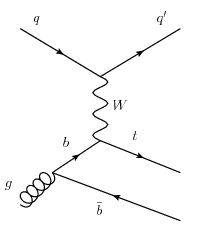
\includegraphics[width=0.25\textwidth]{/afs/ific.uv.es/user/p/pamarag/public/RedaccionTFM/Figuras/singletop_t-ch_2to3.png}
%    \caption{Feynman diagram for $t$-channel production of single top quarks in $pp$ collisions at leading order~\cite{Probin}.}
%    \label{Fig:FeynmanDiagram1}
%\end{figure}
    
%Usual notation \\
%Angles with a * are defined in the $W$-boson reference frame. Angles without the * are defined in the top reference frame. 



\subsection{Top-quark polarisation and W-boson spin observables}\label{subsec:polobs}

In this section we describe the theoretical framework considered in the studies performed in this master thesis, where some of the angular distributions defined in this framework will be considered when designing the selection criteria of an enriched $t$-channel sample at 13~TeV to be used in future measurements of $t$-channel polarisation studies in the LHC Run I.

When produced at hadron colliders, single-top quarks are the only source
of highly polarised top quarks. Specifically, in the $t$-channel, the top quark is produced with a large degree of polarisation in the direction of the spectator quark momentum~\cite{Komm:2014fca}. As the top quark is  extremely unstable, its polarisation must be inferred from the analysis of the angular distributions of the decay products, $W$ and $b$, in the top-quark reference frame. The angular distribution of the charged lepton ($l= e$, $\mu$) from $t \rightarrow Wb \rightarrow l\nu b$ is usually used, because it is the most sensitive to the top-quark polarisation~\cite{CMS:2013rfa}. %<- esta referencia es de CMS y no estás presentando ningún resultado de CMS.


%En la producción de t-channel single top, el quark top tiene un alto grado de polarisación en la dirección del quark espectador. Por lo tanto, se define la dirección del spin del quark top en la dirección del momento del quark espectador en el sistema de referencia del quark top en reposo.


Defining the reference system with axes ($x,y,z$) in the top-quark rest frame, the state of an ensemble of polarised top quarks can be described by a density matrix
\begin{equation} \label{eq:spin-desnity-matrix}
\rho= \frac{1}{2} = \begin{pmatrix} 1+P_z & P_x -iP_y\\ P_x+iP_y & 1-P_z \end{pmatrix}
\end{equation}
where the polarisation in an axis is twice the expected value of the spin in that axis: $P_i=2\langle S_i \rangle$, being $i=x,y,z$. The top-quark spin direction is defined in the direction of the spectator quark momentum in the rest frame of the top quark. The three-dimensional vector $\overrightarrow{P}$ satisfies generally that $|\overrightarrow{P}| \leq 1$, and $|\overrightarrow{P}|=1$ if and only if the quarks are produced as a pure spin state~\cite{AguilarSaavedra:2010nx}. The three orthogonal axis can be taken as: 
\begin{itemize}
\item $\hat{z}$-axis: The direction of the spectator quark three-momentum, $\overrightarrow{p_j}$.
\begin{equation} \label{eq:z-axis}
\hat{z}=\frac{\overrightarrow{p_j}}{|\overrightarrow{p_j}|}
\end{equation}
\item $\hat{y}$-axis: Orthogonal to $\overrightarrow{p_j}$ and the initial quark three-momentum, $\overrightarrow{p_q}$.
\begin{equation} \label{eq:y-axis}
\hat{y}=\frac{\overrightarrow{p_j} \times \overrightarrow{p_q}}{|\overrightarrow{p_j} \times \overrightarrow{p_q}|}
\end{equation}
\item $\hat{x}$-axis: Orthogonal to $\hat{z}$ and $\hat{y}$ and requiring that the coordinate system is right handed.
\begin{equation} \label{eq:x-axis}
\hat{x}=\hat{y}\times \hat{z}
\end{equation}
\end{itemize}

Both vectors, $\overrightarrow{p_j}$ and $\overrightarrow{p_q}$ are measured in the top quark rest frame. The direction of $\hat{z}$ is called \textit{longitudinal}, $\hat{x}$ direction \textit{tranverse} and $\hat{y}$ is the \textit{normal}. It has to be noticed that the momentum direction of the initial quark in the $t$-channel cannot be determined unambiguously in hadronic collisions.% we will deal with this apparent difficulty later.

It is necessary to chose between the two proton beam directions to define the direction of the initial quark in $gq \rightarrow q' t \bar{b}$ so that we can construct the $(x,y,z)$ reference system. To do this, one can use the momentum of the spectator quark in the laboratory frame, which most times follows that of the initial quark (this choice gives the correct answer $97 \%$ times for $ug\rightarrow dt\bar{b}$ and $98 \%$ times for $dg\rightarrow ub\bar{t}$, the main channel for single top and top antiquark production).

For top quark and antiquark we have the following SM polarisations~\cite{AguilarSaavedra:2010nx}:
\begin{align*}
\overrightarrow{P} &\approx (0,0,0.90) & (t) \\
\overrightarrow{P} &\approx (-0.14,0,-0.86) & (\bar{t})
\end{align*}
%Here we arrange the equations in three columns. LaTeX assumes that each equation consists of two parts separated by a &; also that each equation is separated from the one before by an &. 

Those calculus are computed for the $2\rightarrow 3$ process $qg \rightarrow q't\bar{b}$ with the generator PROTOS~\cite{AguilarSaavedra:2008gt}, using CTEQ6L1~\cite{Nadolsky:2008zw} parton distribution functions. The longitudinal agrees with the next-to-leading-order (NLO) calculatios~\cite{Schwienhorst:2010je}; $P_z=0.91$ for quarks and $P_z=-0.86$ for antiquarks. Aditionally, several kinematic distributions are similar~\cite{Campbell:2009ss}. Notice that, in the SM, $P_x$ is not zero for antiquarks because the spectator quark is not the $d$ quarks in the leading production process, $dg \rightarrow ut\bar{b} $ \cite{Mahlon:1996pn}. The presence of new physics in the $t$-channel single-top productions changes completely this SM predictions~\cite{Aguilar-Saavedra:2014eqa}.

\begin{figure} 
\centering
%\subfloat[]{
  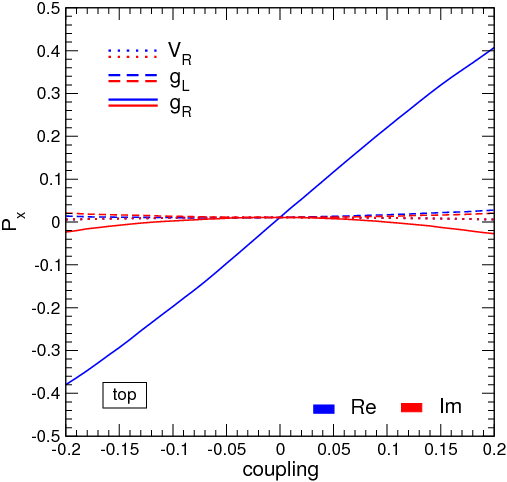
\includegraphics[width=0.3\textwidth]{./Figuras/AGUILARfig1a.png}
%}
%\subfloat[]{
  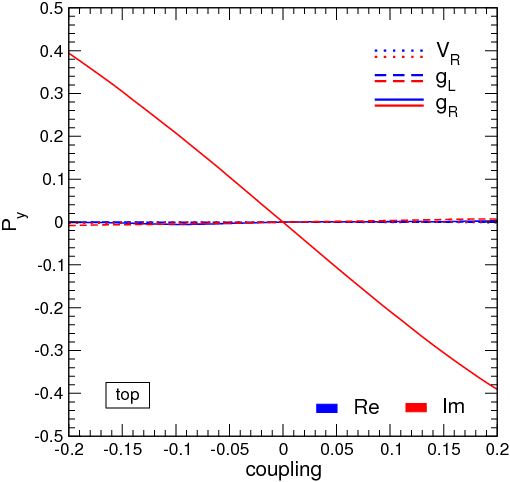
\includegraphics[width=0.3\textwidth]{./Figuras/AGUILARfig1b.png}
%}
%\subfloat[]{
  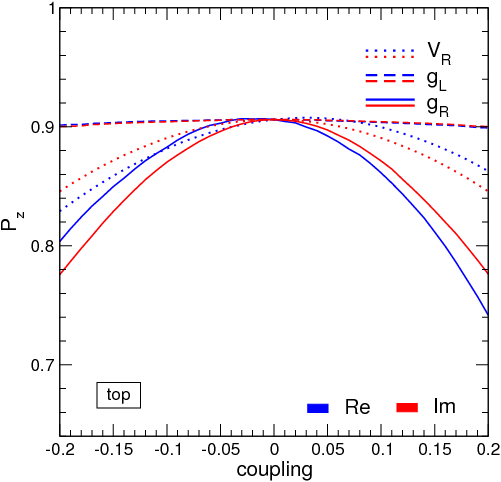
\includegraphics[width=0.3\textwidth]{./Figuras/AGUILARfig1c.png}
%}
\hspace{0mm}
%\subfloat[]{
  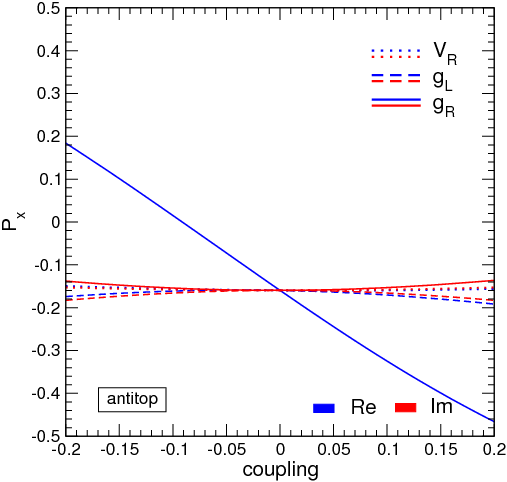
\includegraphics[width=0.3\textwidth]{./Figuras/AGUILARfig1d.png}
%}
%\subfloat[]{   % ???
  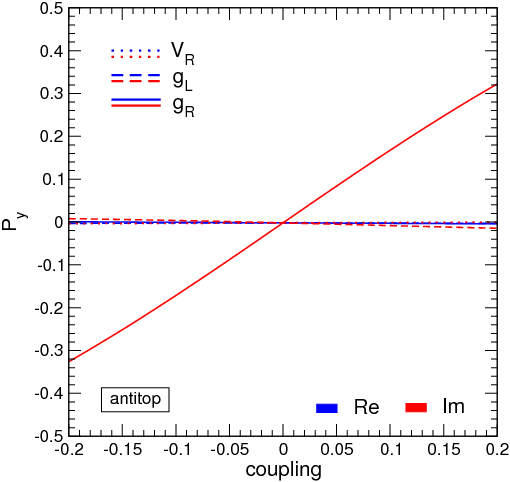
\includegraphics[width=0.3\textwidth]{./Figuras/AGUILARfig1e.png}
%}
%\subfloat[]{
  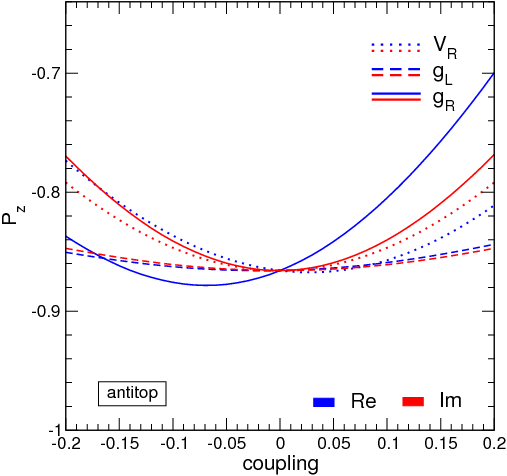
\includegraphics[width=0.3\textwidth]{./Figuras/AGUILARfig1f.png}
%}
\caption{Single top quark (upper row) and antiquark (lower row) polarisation in the axes defined in the equations \eqref{eq:z-axis}, \eqref{eq:y-axis} and \ref{eq:x-axis} as a function of the different coupling constants. The $V_L$ is set to zero~\cite{Aguilar-Saavedra:2014eqa}.} \label{Fig:Polarisation6pack}
\end{figure}

The variations of $P_i$ when a single anomalous coupling from the Lagrangian  \eqref{eq:L_wtb} is non-zero is shown in Figure~\ref{Fig:Polarisation6pack}. The $V_L$ is set to 0 from now on and the range for the anomalous couplings is, according to the order of the current direct limit, $[-0.2,$ $0.2]$. The dependence of the top quark polarisation on anomalous couplings can be extracted from a fit and the resulting expressions are for top quarks~\cite{Aguilar-Saavedra:2014eqa}:
\begin{align*} %\label{eq:Pol-Axis-top
P_x &= (-0.13|V_R|^2+0.25|g_L|^2-0.90|g_R|^2  +2.14 Re\{ V_L^* g_R \} -1.53Re\{ V_R^* g_L \})/f_t \\
P_y &= (-2.12Im\{ V_L^* g_R \} -1.54Im\{ V_R^* g_L \})/f_t \\
P_z &= (0.90 - 0.76|V_R|^2 -1.15|g_L|^{2}-1.50|g_R|^{2}-0.60 Re\{ V_L^* g_R \} +0.36 Re\{ V_R^* g_L \})/f_t
\end{align*}
and for the top antiquarks~\cite{Aguilar-Saavedra:2014eqa}:

\begin{align*} %\label{eq:Pol-Axis-antitop}
P_x &= (-0.14|V_R|^2-0.96|g_L|^2+0.34|g_R|^2 -1.71 Re\{ V_L^* g_R \} +2.31 Re\{ V_R^* g_L \})/f_{\bar{t}} \\
P_y &= (1.72 Im\{ V_L^* g_R \} 2.30 Im\{ V_R^* g_L \})/f_{\bar{t}} \\
P_z &= (-0.86 +0.99 |V_R|^2 -1.56|g_L|^{2}+1.20|g_R|^{2}+0.42Re\{ V_L^* g_R \} - 0.67Re\{ V_R^* g_L \})/f_{\bar{t}}
\end{align*}
Where $f_t$ and $f_{\bar{t}}$ are correction factors for the total corss sections with anomalous couplings~\cite{AguilarSaavedra:2008gt}:
\begin{align*}
f_t &= 1+0.90|V_R|^{2} + 1.47|g_L|^{2}+2.31|g_R|^{2}-0.11Re\{ V_L^* V_R \} - 0.53 Re\{ V_L^* g_R \} \\
f_{\bar{t}} &= 1+1.09|V_R|^{2} + 2.36|g_L|^{2}+1.58|g_R|^{2}-0.12Re\{ V_L^* V_R \} - 0.56 Re\{ V_L^* g_R \}
\end{align*}

The reason for appearance of imaginary parts of coupling products in $P_y$ and not $P_x$ nor $P_z$, can be understood from the $2 \rightarrow 2$ approximation to the $t$-channel. Since the differential cross section is proportional to the square of the modulus of the matrix element, and there are no absorptive parts, those elements can only arise from the traces of Dirac matrices $Tr \{ \gamma^5 \gamma^\mu \gamma^\nu \gamma^\rho \gamma^\sigma \}=-4i\epsilon^{\mu \nu \rho \sigma}$ contracted with four different 4-vectors, being $\epsilon^{\mu \nu \rho \sigma}$ the totally antisymmetric tensor. There are only three independent 4-momenta in the $2 \rightarrow 2$ processes. Therefore, the 4-vector in a non-zero contraction must be the top-spin vector, $\overrightarrow{s_t}$. The Lorentz-invariant contraction $\epsilon_{\mu \nu \rho \sigma}p_q^\mu p_j^\nu p_t^\rho s_t^\sigma$ is proportional to $(\overrightarrow{p_q} \times \overrightarrow{p_j})\cdot \overrightarrow{s_t}$, in the top quark rest frame. The triple product vanishes for $\overrightarrow{s_t}$ in the $\hat{x}$ and $\hat{z}$ but not for the $\hat{y}$ one. This argument is not very affected by the extra $b$ quark in the $2 \rightarrow 3$ process because it is mostly collinear to the beam direction.



%\subsection{polarisation asymmetries} \label{subsec:PolAsym}
%%%%%%%%%%%% Antes esto era otra sección %%%%%%%%%

A study of top-quark physics contributes to the understanding of the origin of the electro-weak symmetry breaking in the SM and its extensions. As mentioned before, the top-quark polarisation is determined from angular distributions of the decay products reconstructed in the top-quark rest frame, while the $W$-boson spin observables are determined from angular distributions of the charged lepton reconstructed in the $W$-boson
rest frame. 
In the top-quark rest frame, the angular distribution of any decay product $X$ of the top quark is given by:
\begin{equation} \label{eq:distrieasy}
\frac{1}{\Gamma}\frac{d\Gamma}{d(\cos \theta_X)}=\frac{1}{2} (1+P \alpha_X \cos \theta_X)
\end{equation}
where $\theta_X$ is the angle between the direction of motion of the decay product in top's rest frame and the top-quark spin axis. $\alpha_X$ is a constant called \textit{spin analysing power} of $X$, $P$ is the top quark degree of polarisation with $0 \leq P \leq 1$ and $\Gamma$ is the total decay width. This $P$ is the one described previously with the components  $P_i=Px$, $P_y$, $P_z$ as defined in equations~\eqref{eq:x-axis}~\eqref{eq:y-axis}~\eqref{eq:z-axis}.

That is, $\alpha_X$ relates the top-quark spin to the angular distribution of the decay product $X$, and it is the fraction of polarisation transferred to the decay products.
The most sensitive spin analyser is the charged lepton; at NLO precision in QCD its spin analysing power is $\alpha_{l^{\pm}} = \pm 0.998$~\cite{Brandenburg:2002xr}. From~\cite{Khachatryan:2015dzz} can be calculated the product of the top momentum and the spin analysing power of the lepton which is $P\cdot \alpha_{\mu} = 0.58 \pm 22$ for the top and $P\cdot \alpha_\mu = 0.42 \pm 28$ for the anti-top. The combination of both is $P\cdot \alpha_\mu = 0.52 \pm 22$. %Decir que esto es con CMS
%Creo que esta escho considerando el muon como lepton



From the spin density matrix in Equation~\eqref{eq:spin-desnity-matrix}, $W$-boson helicity components 0 and $\pm 1$ resulting from the decay of  polarised top-quarks, can be parameterised in terms of expectation values of six independent spin observables~\cite{Probing} $\langle S_{1, 2, 3} \rangle$, $\langle A_{1, 2} \rangle$ and $\langle T_{0} \rangle$. The polar and azimuthal angles of the charged lepton in the $W$-boson rest frame are denoted by $\theta^{*}_l$ and $\phi^{*}_l$; from now on, the variables with the star ($^{*}$) are in the $W$-boson rest frame. The fully differential decay width of $W$ can be written as:
%\begin{align} 
%\frac{1}{\Gamma}\frac{d\Gamma}{d(\cos \theta_l^{*})d\phi_l^{*}}&=\frac{3}{8 \pi} \Big \{ \frac{3}{2}+\frac{1}{\sqrt{6}} \langle T_{0} \rangle (3 \cos^{2}\theta_l^{*}-1)+ \langle S_{3} \rangle \cos\theta_l^{*} \\ &+ \langle S_{1} \rangle \cos\phi_l^{*} \sin\theta_l^{*} +  \langle S_{2} \rangle \sin\phi_l^{*} \sin\theta_l^{*} \\ &- \langle A_{1} \rangle \cos\phi_l^{*} \sin2\theta_l^{*} - \langle A_{2} \rangle \sin\phi_l^{*} \sin2\theta_l^{*} \Big \} 
%\end{align} \label{eq:angdist}

\begin{equation} \label{eq:angdist}
\begin{split}
 \frac{1}{\Gamma}\frac{d\Gamma}{d(\cos \theta_l^{*})d\phi_l^{*}} = & \frac{3}{8 \pi} \Big \{ \frac{3}{2}+\frac{1}{\sqrt{6}} \langle T_{0} \rangle (3 \cos^{2}\theta_l^{*}-1)+ \langle S_{3} \rangle \cos\theta_l^{*} \\
 & + \langle S_{1} \rangle \cos\phi_l^{*} \sin\theta_l^{*} +  \langle S_{2} \rangle \sin\phi_l^{*} \sin\theta_l^{*} \\
 & - \langle A_{1} \rangle \cos\phi_l^{*} \sin2\theta_l^{*} - \langle A_{2} \rangle \sin\phi_l^{*} \sin2\theta_l^{*} \Big \} 
\end{split}
\end{equation} 

In this formalism the $W$-boson spin axis is taken along the direction of the $W$-boson momentum in the top-quark rest frame, or equivalently along the direction opposite to the $b$-quark momentum in the $W$-boson rest frame. In Figure~\ref{Fig:CoordSyst} can be seen the coordinate system used and the various angles defined for the charged lepton in the $W$ rest frame.  Here, the axis are defined as follows: $\hat{z}$ is the $W$-boson momentum direction in the top-quark rest frame; the direction of top's spin, $\hat{s_t}$, taken along the spectator quark momentum in top quark rest frame defines the $\hat{x}$-$\hat{z}$ plane. The momentum of the charged lepton is $\overrightarrow{p_l}$ in the $W$ rest frame. The normal and transverse axes are defined relatively to $\overrightarrow{q}$ and $\hat{s_t}$ according to $\overrightarrow{N}= \hat{s_t} \times \overrightarrow{q}$ and $\overrightarrow{T}= \overrightarrow{q} \times \overrightarrow{N}$; they are along the $-\hat{y}$ and $\hat{x}$ axes of the coordinate system, respectively. The azimuthal angles of the charged lepton in the $W$-boson rest frame ($\phi_N^{*}$,$\phi_T^{*} \equiv \phi_l^{*}$) are defined relatively to the $\overrightarrow{N}$ and $\overrightarrow{T}$ axes while $\theta_l^{N}$ and $\theta_l^{T}$, which are not showm in the Figure~\ref{Fig:CoordSyst}, are the relative angles between the $\overrightarrow{N}$ and the $\overrightarrow{T}$ and axes respectively.

\begin{figure}[htb]
\centering
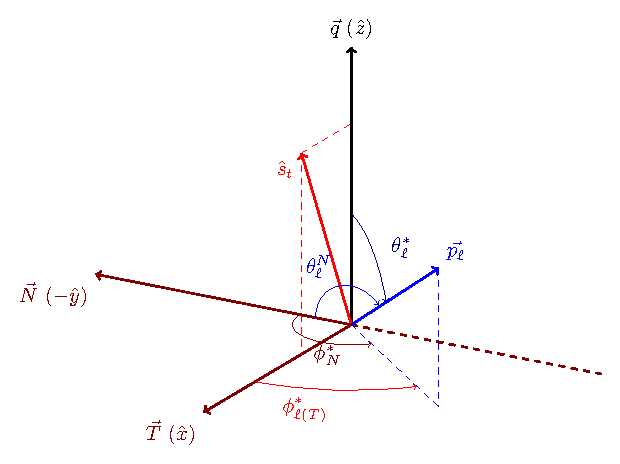
\includegraphics[width=0.85\textwidth]{/afs/ific.uv.es/user/p/pamarag/public/RedaccionTFM/Figuras/coord_system_pol.pdf}
\caption{Coordinate system and angles used to define the $W$-boson spin observables and their related angular asymmetries in the decay of polarised top quarks.}
\label{Fig:CoordSyst}
\end{figure}

There is an integral over all the possible direction of the top-quark spin relative to the $W$-boson spin axis implied by the angular distribution of equation~\eqref{eq:angdist}. The polarisation of the top quark is propagated to the spin observables $\langle S_{1, 2} \rangle$ and $\langle A_{1, 2} \rangle$, which are proportional to $P$. The other spin observables $\langle S_{3} \rangle$ and $\langle T_{0} \rangle$ are not depending on $P$ and are related to the $W$-boson helicity fractions: $F_R$, $F_L$ and $F_0$~\cite{Aguilar-Saavedra:2015yza}.

Using the SM predictions of the helicity fractions at next-to-next-leading-order (NNLO) in QCD, assuming a top mass of $172.5$ GeV and a $b$-quark mass of 4.8 GeV~\cite{Czarnecki:2010gb}, it is found that $\langle S_{3} \rangle = -0.31 \pm 0.01$ and $\langle T_{0} \rangle = -0.43 \pm 0.01$. The polarisation-dependent spin observables can be obtained combining the predicted degrees of polarisation ($P_t= 0.91$ and $P_{\bar{t}}=-0.86$) with the $t$-channel single-top cross sections ($\sigma_t = 54.9$ pb and $\sigma_{\bar{t}}=29.7$ pb) calculated at NLO in QCD. Then, the SM predictions calculated at LO in QCD for $\langle S_{1, 2} \rangle$ and $\langle A_{1, 2} \rangle$ are: $\langle S_{1} \rangle=0.46\pm 0.01$, $\langle A_{1} \rangle = 0.23\pm 0.01$ and $\langle S_{2} \rangle = \langle A_{2} \rangle = 0.00\pm 0.01$~\cite{Probing}. If the measured values of $\langle S_{2} \rangle$ and $\langle A_{2} \rangle$ spin observables were different of zero, it would imply the presence of an imaginary coupling in the $Wtb$ vertex (eq.~\eqref{eq:L_wtb}) since those observables are only sensitive to Im$\{ g_R \}$~\cite{Probing}. The observable $\langle S_{2} \rangle$ is twice ar sensitive as $\langle A_{2} \rangle$ to Im$\{ g_R \}$, which makes it more suitable for determining this coupling. The other four $W$-boson spin observables are mainly sensitive to Re$\{ g_R \}$, having a poor sensitivity to Im$\{ g_R \}$. %The existence of Im$\{ g_R \} \neq 0$ would imply $\mathcal{CP}$ violation.
%There are in total 6 spin observables: 2 of them are sensitive to Im{g_R}.


The $W$-boson spin observables and top-quark polarisation can be extracted from asymmetries derived by integrating the angular distributions expressed in equations \eqref{eq:distrieasy} and \eqref{eq:angdist}. These asymmetries are based on single or combined angular observables. A list of the asymmetries, their associated angular observables, their relation to the polarisation observables and their values predicted by the SM can be found on Table \ref{table:Asymmetries}.

\begin{table}
\renewcommand{\arraystretch}{1.3}
\begin{tabular}{|c c c c|} 
\hline
Asymmetry & Angular Observable & polarisation observable & SM prediction $(\pm 0.01)$ \\
\hline
$A_{FB}^{l}$ & $\cos \theta_{l}$ & $\frac{1}{2}\alpha_l P$ & 0.45\\

$A_{FB}^{tW}$ & $\cos \theta_{W}\cos \theta_{l}^{*}$ & $\frac{3}{8}P(F_R + F_L)$ & 0.10\\

$A_{FB}$ & $\cos \theta_{l}^{*}$ & $\frac{3}{4}\langle S_3 \rangle=\frac{3}{4}(F_R - F_L)$ & -0.23\\

$A_{EC}$ & $\cos \theta_{l}^{*}$ & $\frac{3}{8} \sqrt{\frac{3}{2}}\langle T_0 \rangle=\frac{3}{16}(1 - F_0)$ & -0.20\\

$A_{FB}^T$ & $\cos \theta_{l}^{T}$ & $\frac{3}{4}\langle S_1 \rangle$ & 0.34\\

$A_{FB}^{N}$ & $\cos \theta_{l}^{N}$ & $-\frac{3}{4}\langle S_2 \rangle$ & 0\\

$A_{FB}^{T,\phi}$ & $\cos \theta_{l}^{*}\cos \phi_{T}^{*}$ & $-\frac{2}{\pi} \langle A_1 \rangle$ & -0.14\\

$A_{FB}^{N,\phi}$ & $\cos \theta_{l}^{*}\cos \phi_{N}^{*}$ & $\frac{2}{\pi} \langle A_2 \rangle$ & 0\\
\hline

\end{tabular}
\caption{Asymmetries with their associated angular observables and their relation to the top-quark polarisation and $W$-boson spin observables.}
\label{table:Asymmetries}
\end{table}

The forward-backward (FB) asymmetry, in which most polarisation observables used here are based on, is defined as a function of a given angular observable $\cos \theta$ according to
\begin{equation}
A_{FB}=\frac{N(\cos\theta > 0)-N(\cos\theta < 0)}{N(\cos\theta > 0)+N(\cos\theta < 0)}
\end{equation}
where $N$ is the number of events. For the $W$, the other used asymmetry is the so called edge-central (EC), which is similarly defined
\begin{equation}
A_{EC}=\frac{N(\cos\theta > \frac{1}{2})-N(\cos\theta < \frac{1}{2})}{N(\cos\theta > \frac{1}{2})+N(\cos\theta < \frac{1}{2})}
\end{equation}

The asymmetry $A_{FB}^{l}$ allows us to determine the product $\alpha_l P$ from the angular distribution $\cos \theta_l$, being $\theta_l$ the angle between the lepton momentum in the top quark rest frame and the top-quark spin axis. From the $A_{FB}^{tW}$ is possible to obtain $P$; this asymmetry is defined with respect to the combined angular observable $\cos \theta_{W}\cos \theta_{l}^{*}$ (see Table \ref{table:Asymmetries}), where $\theta_W$ is the angle between the $W$-boson momentum in the top-quark rest frame and the top-quark spin axis. The $W$-boson spin observables $\langle S_{3} \rangle$ and $\langle T_{0} \rangle$ are derived from the forward-backward asymmetry $A_{FB}$ and from the edge-central asymmetry $A_{EC}$ of the $\cos \theta_l^{*}$ angular distribution, respectively. The $\langle S_{1} \rangle$ and $\langle S_{2} \rangle$ are determine from $A^T_{FB}$ $A^N_{FB}$ in the angular observables $\cos \theta_l^T$ and $\cos \theta_l^N$, respectively. The spin observables $\langle A_{1} \rangle$ and $\langle A_{2} \rangle$ are extracted from $A_{FB}^{T,\phi}$ and $A_{FB}^{N,\phi}$. This is based on the $W$-boson helicity, $\cos\theta_l^{*}$, multiplied per the cosine of $\phi_{T}^{*}$ and $\phi_{N}^{*}$ defined with respect to $\overrightarrow{T}$ and $\overrightarrow{N}$, respectively.

The asymmetry $A_{FB}^{N}$ is very sensible to the coupling $g_R$, therefore it can be used to extract limits on Im$\{g_r \}$. Considering small values of Im$\{g_r \}$ and taking $V_L =1$ and $v_R=g_L=0$, a linear dependence of the form $A^N_{FB}=0.64\cdot P \cdot$Im$\{g_r \}$ is obtained~\cite{AguilarSaavedra:2010nx}. As $A^N_{FB}$ depends on $P$, the measured value of the $A^l_{FB}$ asymmetry is required to constrain $P$ for the limit computation. %No se si podar información de aquí


